\documentclass[11pt]{article}

\usepackage[utf8]{inputenc}
\usepackage[T1]{fontenc}
\usepackage{mathpazo} % Palatino font
\usepackage{microtype}
\usepackage{amsmath, amssymb, amsthm}
\usepackage{geometry}
\geometry{a4paper, margin=1.2in}
\usepackage{algorithm}
\usepackage{algpseudocode}
\usepackage[backend=biber,style=numeric,sorting=none,natbib=true]{biblatex}
\addbibresource{references.bib}
\usepackage{hyperref}
\usepackage{xcolor}
\usepackage{bm}
\usepackage{graphicx}

\hypersetup{ colorlinks=true, linkcolor=blue!60!black, citecolor=green!50!black, urlcolor=blue!60!black
}

\title{Empirical Bayes-augmented convex matrix factorization, completion and denoising}
\author{David A Knowles}
\date{}

\begin{document}

\maketitle

\begin{abstract}
Typical matrix factorization and completion models involve non-convex optimization, so that different initialization or small perturbations to the data can give grossly different solutions. An elegant alternative is to estimate an underlying low-rank ``clean'' data matrix by enforcing it have small nuclear norm (the convex envelope of matrix rank). This convex optimization problem can be efficiently solved using proximal gradient or Franke-Wolfe methods. However, choosing the regularization strength typically requires cross-validation, involving arbitrary choices (e.g., number of folds), randomness, and substantial computation. Here, we propose empirical Bayes approaches to selecting the regularization strengh, using the recently characterized nuclear norm distribution. We consider multiple noise models, including homoskedastic, known heteroskedastic, and a combination thereof. We present results on simulated data, genetic associations, and single-cell splicing patterns. 
\end{abstract}

\tableofcontents

\section{Introduction}

Low-rank matrix factorization is a workhorse of modern data analysis, underpinning methods ranging from recommender systems to single cell genomics. Yet the overwhelming majority of factorization approaches including non-negative matrix factorization, independent component analysis, and sparse Principal Component Analysis (PCA), optimize a non-convex objective over a product of factor matrices. Non-convexity has practical consequences: different random initializations or minor data perturbations can result in methods finding qualitatively different local minima, making results difficult to reproduce and the recovered factor structure ambiguous \citep{lee1999learning, cai2021}. Classical PCA is the notable exception, enjoying a globally optimal and unique solution (up to sign flips) via the singular value decomposition, but it cannot handle missing data or heteroskedastic noise, and it provides no internal mechanism for selecting the rank of the solution.

Convex relaxations offer a principled escape from local minima. The nuclear norm, the convex envelope of matrix rank, yields a globally convex objective that implicitly encourages low-rank solutions without factorizing the data matrix \citep{recht2010guaranteed, candes2010power}. Solving the nuclear-norm-regularized problem produces a unique, reproducible answer regardless of initialization. A practical difficulty, however, is that the strength of the regularization must be chosen by the analyst. Cross-validation (CV) is the standard remedy, but it is computationally expensive and requires arbitrary choices about the CV scheme (e.g., the number of folds and how to choose heldout matrix elements). 

We resolve both limitations simultaneously through an empirical Bayes framework. By interpreting the nuclear norm penalty as the negative log-prior of a \emph{nuclear norm} distribution and placing an uninformative Gamma hyperprior on the regularization strength $\lambda$, we obtain a Bayesian interpretation in which $\lambda$ is estimated from the data alongside the latent matrix $X$. Crucially, a naive maximum a posteriori (MAP) approach fails here due to the Neyman–Scott paradox: collapsing posterior uncertainty into a point estimate causes the effective nuclear norm to be underestimated, biasing $\lambda$ upward and over-shrinking the signal. We sidestep this by developing a Coordinate Ascent Variational Inference (CAVI) algorithm that maintains explicit posterior uncertainty over $X$, leading to well-calibrated automatic regularization without any cross-validation.

\section{Model}

\subsection{Homoskedastic setup}

For exposition, we first consider a homoskedastic noise model. Assume we observe elements $\Omega \subseteq \{1,\ldots,m\}\times\{1,\ldots,n\}$ of a noisy data matrix $Y$. We aim to find a ``denoised'' low-rank matrix $X$ close to $Y$ (e.g., in squared error). The typical approach would be to represent $X=UV^T$ and optimize over $U$ and $V$, but this is non-convex and requires careful initialization. 

\paragraph{Convex optimization formulation.} In the convex optimization/compressed sensing literature, a common alternative is to place a convex penalty directly on $X$ that encourages low-rank structure. The natural choice is the nuclear norm $\|X\|_* = \sum_i s_i(X)$, the sum of the singular values (SVs) $s$ of $X$. The loss is then, 
\begin{equation} \label{eq:loss} \mathcal{L}(X) = \frac12 \sum_{ij \in \Omega} (Y_{ij}-X_{ij})^2 + \lambda \|X\|_*.
\end{equation}
In principle $\lambda$ can be selected by CV, but this is computationally expensive and requires arbitrary choices about the CV scheme (how many folds, how to select heldout entries, what metric to use). 

Eq \eqref{eq:loss} can be efficiently solved using proximal gradient updates. Split \eqref{eq:loss} into a smooth part $h(X) = \frac12 \sum_{ij \in \Omega} (Y_{ij}-X_{ij})^2 $ and the nonsmooth nuclear-norm term $\lambda\|X\|_*$.  The proximal-gradient step is
\begin{align} Z^{(t)} = X^{(t)} - \alpha_t\nabla h(X^{(t)}), \qquad X^{(t+1)} = \operatorname{SVT}_{\alpha_t\lambda}\!\left(Z^{(t)}\right), \label{eq:proxgrad}
\end{align}
where $\operatorname{SVT}_\tau$ soft-thresholds the singular values by $\tau$.
The step size $\alpha_t$ is selected by backtracking until
$\mathcal{L}(X^{(t+1)})\leq\mathcal{L}(X^{(t)})$.

\paragraph{Bayesian interpretation.} Here, we ask whether Eq \ref{eq:loss} can be re-interpreted from an (empirical) Bayesian viewpoint to enable automatic estimation of $\lambda$ from the data. The squared error loss can be interpreted as the (scaled) log pdf of a Gaussian likelihood, 
\begin{align} Y_{ij} \mid X_{ij}, \sigma &\sim \mathcal{N}(X_{ij}, \sigma^2), \qquad (i,j)\in\Omega,
\end{align}
where $\sigma^2$ is the noise variance. 
%While it might be appealing to think of $g=1$, we will see it is preferable to think of $\lambda$ as absorbing $g$ 
We consider the nuclear norm penalty as the negative log-pdf of the recently characterized\cite{Segert2025-rk} \emph{nuclear norm distribution} (NND), 
\begin{equation} p(X \mid \eta) = \frac{1}{Z(\eta)} \exp\big(-\eta \|X\|_*\big)
\end{equation}
where the normalizing constant $Z(\eta)=(mn)! C / \eta^{mn}$, with $C$ the volume of the unit nuclear norm ball. 
\citet{Segert2025-rk} proved that setting the NND rate $\eta = \lambda/\sigma$ (and the prior on $\sigma^2$ being log-concave in $1/\sigma$) ensures that $P(X,\sigma|Y,\lambda)$ is unimodal.

\subsection{Limitations of full Bayesian inference for the NND}

\paragraph{Inference challenges.} \citet{Segert2025-rk} use Markov chain Monte Carlo (MCMC) to sample $X$, $g$ and $\lambda$ under this model. While statistically rigorous, the MCMC is computationally painful, requiring full SVDs at each iteration and tedious tuning to obtain reasonable mixing. We also explored a coordinate ascent variational inference (CAVI) approach using a lesser-known bound for the nuclear norm that introduces an auxiliary covariance parameter (see Appendix \ref{app:cavi}). Thehe CAVI algorithm is more computationally efficient, but takes us back to a non-convex optimization problem (although arguably with a better behaved optimization landscape than naive matrix factorization, e.g., we are able to show contraction to a single optimum under certain conditions, see Appendix \ref{app:contraction}). Even stochastic variational inference offers no panacea: any reasonable variational approximation immediately reintroduces the non-convexity we are trying to avoid. 

\paragraph{Prior behavior.} \citet{Segert2025-rk} showed that $X \sim NND(\eta)$ is equal in distribution to $X = U \text{diag}(s) V$ where $U$ and $V$ are sampled uniformly from the space of orthonormal matrices, and, assuming (without loss of generality) $m \ge n$, the joint density of the non-zero SVs $s_1 > s_2 > \dots > s_n > 0$ is, 
\begin{equation} p(s_1, \dots, s_n) \propto \prod_{i=1}^n \underbrace{ s_i^{m-n} e^{-\eta s_i}}_{\propto \, \mathrm{Gamma}(m-n+1,\,\eta)} \cdot \underbrace{\prod_{1 \le i < j \le n} (s_i^2 - s_j^2)}_{\text{repulsion term}}
\label{eq:nnd-sv-distribution}
\end{equation}
This distribution on the SVs of $X$ is concerning for $m > n$ since the shape $m-n+1 > 1$ means that the SVs are pushed\ \emph{away} from $0$. This is analogous to the Lasso, where optimization under the L1 penalty gives sparse solutions, but Bayesian inference under the analogous Laplace prior does not (motivating spike-and-slab priors, despite their fitting challenges). Note that sparser priors on the SVs would result in non-convex optimization. 

\begin{figure}
\centering
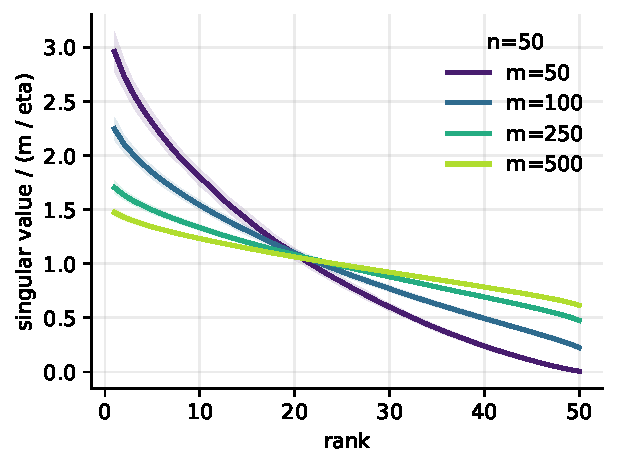
\includegraphics[width=0.6\textwidth]{figures/nnd_sv_profiles_scaled.pdf}
\caption{Expected SV profiles under the NND, obtained by NUTS applied to Eq \eqref{eq:nnd-sv-distribution}. Especially for $m \gg n$, the NND pushes SVs away from zero, which is undesirable for regularization.}
\end{figure}

\subsection{A hybrid solution: convex optimization and empirical Bayes}

Given this fundamental mismatch of full Bayesian inference with the NND model we instead explore a hybrid solution. We use the convex optimization machinery of proximal gradient to learn $X$ (MAP) solutions over a grid of $\eta$ (effective regularization) values. We then derive a closed form variational approximation centered on $X$ via a Taylor series expansion of the expected nuclear norm. This lets us learn the noise variance $\sigma^2$ (and implicitly the NND rate $\lambda = \eta \sigma$) via maximum marginal likelihood (i.e. empirical Bayes). The grid of $X$ solutions can then be evaluated by approximate marginal likelihood or leave-one-out (LOO) scores, which are available in closed form given the variational covariance. 

We note that we found that joint optimization of the approximate ELBO for $\lambda$ and $\sigma$ was unstable.

\subsection{Approximating the marginal likelihood with variational inference}

We assume a row-factorized Gaussian approximation $ q(X) = \prod_{i=1}^m \mathcal{N}(x_i\mid \mu_i,\Sigma_i)$ where $x_i$ is row $i$ of $X$. To cover both the homoscedastic model here and the heteroscedastic models below, we introduce effective noise precisions $p_{ij}$, with $p_{ij} = 1/\sigma^2$ for $(i,j)\in\Omega$ (for the homoscedastic case) and $0$ otherwise. The evidence lower bound (ELBO) is,
\begin{align} \mathcal{L}(\mu,\Sigma) &= -\frac{1}{2} \sum_{i=1}^m \left[ (y_i-\mu_i)^\top P_i (y_i-\mu_i) + \operatorname{tr}(P_i\Sigma_i) \right] + \frac{1}{2}\sum_{i=1}^m \log|\Sigma_i| + \frac12 \sum_{(i,j)\in\Omega}\log p_{ij} \notag\\ &\quad - \eta\mathbb{E}_q\|X\|_* - \log Z(\eta) + \mathrm{const}, \label{eq:full-elbo}
\end{align}
where $P_i = \text{diag}\{p_{i:}\}$ is the diagonal precision matrix for row $i$. The difficulty is $\mathbb{E}_q\|X\|_*$.  Write
$X=\mu+E$ with $\mathbb{E}_q(E)=0$ and
$\mathbb{E}_q(E^\top E)=\sum_i\Sigma_i$.  Using the trace identity
$\|X\|_*=\operatorname{tr}\{(X^\top X)^{1/2}\} =: f(X^\top X)$, where
\begin{equation} X^\top X = \mu^\top\mu + \mu^\top E + E^\top\mu + E^\top E.
\end{equation}
Expanding $f$ around $\mu^\top\mu$ and taking expectations, the
linear terms $\mu^\top E+E^\top\mu$ vanish.  Keeping the dominant covariance
term gives the matrix-delta approximation
\begin{equation} \mathbb{E}_q\|X\|_* \approx \|\mu\|_* + \frac{1}{2} \operatorname{tr} \left[ B(\mu) \sum_{i=1}^m \Sigma_i \right]. \label{eq:taylor-expected-nuc}
\end{equation}
where $B(\mu) = (\mu^\top\mu+\epsilon I)^{-1/2}$. The small ridge $\epsilon I$ stabilizes the inverse square root when $\mu$ is
rank deficient. Substituting \eqref{eq:taylor-expected-nuc} into \eqref{eq:full-elbo}, the terms involving a single row covariance are,
\begin{equation} \mathcal{L}_i(\Sigma_i) = \frac{1}{2}\log|\Sigma_i| - \frac{1}{2} \operatorname{tr} \left[ \{P_i+\eta B(\mu)\}\Sigma_i \right] + \mathrm{const}.
\end{equation}
Taking a matrix derivative and setting it to zero gives the optimum,
\begin{align}
A_i = P_i+\eta B(\mu), \qquad \hat{\Sigma}_i = A_i^{-1}. \label{eq:taylor-row-precision}
\end{align}
Because $\Sigma_i$ has this closed-form optimum given $\mu$, it can be substituted
back into the ELBO.  The trace term collapses to a constant
$-\frac{1}{2}\operatorname{tr}(I_n)$ per row, leaving the collapsed ELBO,
\begin{align} \mathcal{L}_{\mathrm{Taylor}}(\mu) &= -\frac{1}{2} \sum_{(i,j)\in\Omega} p_{ij}(Y_{ij}-\mu_{ij})^2 - \eta\|\mu\|_* - \frac{1}{2}\sum_{i=1}^m \log |A_i| \notag\\ &\quad + \frac12 \sum_{(i,j)\in\Omega}\log p_{ij} + mn\log\eta + \text{noise-prior terms}. \label{eq:taylor-elbo}
\end{align}
Here we used that $\log Z(\eta)=-mn\log\eta+\mathrm{const}$.

One might be tempted to fit $\mu$ by maximizing \eqref{eq:taylor-elbo}. However this is 1) computationally challenging at $O(nm^3)$ given the sum of log determinants terms 2) non-convex and 3) statistically ill-advised given the arguments above regarding the downsides of the full Bayesian model. 

\subsection{Optimization}

For the implemented version we use an inverse-gamma variance prior,
\begin{equation} p(\sigma) \propto \sigma^{-(a_0+1)}\exp(-b_0/\sigma),
\end{equation}
although the objective separates the prior contribution so that another one-dimensional prior on $\sigma$ can be substituted. Ideally this should be log-concave in $1/\sigma$ to ensure unimodality of the posterior.

\paragraph{Scoring.} Our default strategy is to score solutions using the ELBO \eqref{eq:taylor-elbo} evaluated at the proximal mean $\hat X$ and the optimal covariance $\hat \Sigma_i$ given by \eqref{eq:taylor-row-precision}. However, the same covariance gives an analytical leave-one-entry-out (LOO) score.  If
$r_{ij}=p_{ij}\Sigma_i[j,j]$, then for observed entries
\begin{equation} \log p^{\mathrm{LOO}}(Y_{ij}) = -\frac{p_{ij}(Y_{ij}-\hat X_{ij})^2}{2(1-r_{ij})} -\frac{1}{2}\log(2\pi/p_{ij}) +\frac{1}{2}\log(1-r_{ij}).
\end{equation}
The LOO score is the sum of these terms over $\Omega$.

\subsection{Known heteroskedastic noise}

Here, we consider known standard errors $\Delta \in \mathbb{R}^{m \times n}$, where $\delta_{ij}$ is the uncertainty associated with $Y_{ij}$, 
\begin{align}
Y_{ij} \mid X_{ij}, \delta_{ij} &\sim \mathcal{N}(X_{ij}, \delta_{ij}^2), \qquad (i,j)\in\Omega.
\end{align}
In the notation of Eq \eqref{eq:full-elbo}, the precision $p_{ij} = 1/\delta_{ij}^2$ for $(i,j)\in\Omega$ and $0$ otherwise. The proximal gradient update is the same as in the homoskedastic case, but with a weighted squared error loss. The ELBO is also the same with the appropriate precision terms. Since the noise is known, there is no noise variance to update, so the only hyperparameter is $\lambda$, which is scored by ELBO or LOO over a grid of possible values. 

\subsection{Unknown homoskedastic plus known heteroskedastic noise}

In some settings, we have a combination of known heteroskedastic noise and unknown homoskedastic noise. For example, in single-cell RNA-seq data, we might model the observed counts as subject to both count noise (known heteroskedastic) and other technical noise (unknown homoskedastic). In this setting, the effective precision is $p_{ij} = 1/(\delta_{ij}^2 + \sigma^2)$ for $(i,j)\in\Omega$ and $0$ otherwise. 

For this variant, $\hat{X}=\mu$ and the noise variance $\sigma^2$ are coupled, so we update them by alternating steps. For the mean update we use the proximal gradient step Eq \eqref{eq:proxgrad}, with $\eta = \lambda/\sigma$, where $\sigma^2$ is the current noise variance estimate. After the mean update, the scalar variance is updated on the unconstrained scale $\ell=\log \sigma$ by a gradient step on the negative ELBO \eqref{eq:taylor-elbo}, again with backtracking to enforce monotonicity. 



\printbibliography

\section{Appendix}

\subsection{Coordinate Ascent Variational Inference (CAVI)}

Our key insight to enable CAVI is that the nuclear norm can be expressed as a minimization over an auxiliary symmetric positive definite matrix $Q \in \mathbb{S}_{++}^n$,
\begin{equation} \|X\|_* = \min_{Q \succ 0} \frac{1}{2} \text{Tr}(X Q^{-1} X^T) + \frac{1}{2} \text{Tr}(Q).
\end{equation}
Augmenting the optimization with $Q$ and applying Jensen's inequality gives a tractable bound on the nuclear norm term of the ELBO: 
\begin{equation} \mathbb{E}_{q}[-\lambda \|X\|_*] \ge -\frac12 \lambda \mathrm{Tr}\!\left(\mathbb{E}_{q}[X^T X]\, Q^{-1}\right) - \frac12 \lambda \mathrm{Tr}(Q).
\end{equation}
and naturally results in $q(X)$ factorizing over rows of $X$. Given the symmetry of the nuclear norm, there is an alternative representation with $Q \in \mathbb{S}_{++}^m$ and $X^T Q^{-1} X$, which would result in a column-wise factorization of $q(X)$. The choice between these is a matter of computational convenience: the row factorization is more efficient when $m \gg n$ and the column factorization is more efficient when $n \gg m$. 

\paragraph{Update for $q(X)$.} Given $Q$ and $\lambda$, the posterior for each row $x_i$ is a multivariate Gaussian, i.e. $q(X) = \prod_{i=1}^m \mathcal{N}(x_i \mid \mu_i, \Sigma_i)$, with mean and covariance given by
\begin{align} \Sigma_i &= \left( P_i + \lambda Q^{-1} \right)^{-1}, \qquad \mu_i = \Sigma_i \left( P_i y_i \right)
\end{align}
The auxiliary matrix $Q$ induces correlation across the columns of $X$. 

\paragraph{Update for Auxiliary Matrix $Q$.} Let $\Psi = \mathbb{E}_{q}[X^T X] = \sum_{i=1}^m (\mu_i \mu_i^T + \Sigma_i)$. The value of $Q$ that tightly bounds the expectation is the matrix square root $Q^* = \Psi^{1/2}$. 

\paragraph{Update for NND rate $\lambda$.} In principle we could update $\lambda$ analytically under a conjugate Gamma prior. However, we generally find is it preferable to treat $\lambda$ as a hyperparameter and select it by maximizing the ELBO or LOO score over a grid of values.

\paragraph{Batched implementation.} For settings where $n$ is moderate (e.g.\ $n \lesssim 300$) but $m$ is large, the bottleneck of full CAVI is the simultaneous storage of all $m$ row covariances $\Sigma_i \in \mathbb{S}_{++}^n$. We address this using mini-batches of size $B$. Each batch computes $\Sigma_i$ via Cholesky, immediately extracts $\mathrm{diag}(\Sigma_i)$ (needed for the ELBO) and the batch's contribution to $\Psi = \sum_i (\mu_i\mu_i^\top + \Sigma_i)$, then discards the full $\Sigma_i$ before moving to the next batch. Peak memory is $O(Bn^2 + mn)$ rather than $O(mn^2)$. 

\end{document}
